\documentclass{article}

\usepackage[left=2cm,right=2cm,top=2cm,bottom=2cm]{geometry} 

\usepackage[utf8]{inputenc}   % otra alternativa para los caracteres acentuados y la "ñ"
\usepackage[           spanish % para poder usar el español
                      ,es-tabla % para los captions de las tablas
                       ]{babel}   
\decimalpoint %para usar el punto decimal en vez de coma para los números con decimales

%\usepackage{beton}
%\usepackage[T1]{fontenc}

\usepackage{parskip}
\usepackage{xcolor}

\usepackage{caption}

\usepackage{fancyvrb}

\usepackage{enumerate} % paquete para poder personalizar fácilmente la apariencia de las listas enumerativas

\usepackage{graphicx} % figuras
\usepackage{subfigure} % subfiguras

\usepackage{amsfonts}
\usepackage{amsmath}

\usepackage[formats]{listings}
\lstdefineformat{R}{~=\( \sim \)}
\lstset{basicstyle=\ttfamily,format=R}

\definecolor{gris}{RGB}{220,220,220}
	
\usepackage{float} % para controlar la situación de los entornos flotantes

\restylefloat{figure}
\restylefloat{table} 
\setlength{\parindent}{0mm}


\usepackage[bookmarks=true,
            bookmarksnumbered=false, % true means bookmarks in 
                                     % left window are numbered
            bookmarksopen=false,     % true means only level 1
                                     % are displayed.
            colorlinks=true,
            allcolors=blue,
            urlcolor=blue]{hyperref}
\definecolor{webblue}{rgb}{0, 0, 0.5}  % less intense blue


\title{\Huge SWAP: Balanceo de carga en un sitio web\vspace{10mm}}

\author{\huge David Cabezas Berrido \vspace{10mm} \\ 
  \huge dxabezas@correo.ugr.es \vspace{10mm}}

\begin{document}
\maketitle
\tableofcontents
\newpage

\section{Preparativos}

Creamos dos archivos \texttt{/var/www/html/index.html} básicos en las máquinas 1 y 2, donde se referencie el número de la máquina a la que
pertenece el archivo para saber cuál de las dos máquinas atendió la petición.

Creamos una nueva máquina virtual M3 con Ubuntu Server, pero no instalamos los servicios de la práctica 1, ya que no podemos
tener a Apache ocupando el puerto 80. Nos limitamos a configurar el doble
adaptador de red como hicimos en las otras dos máquinas. Su dirección IP es 192.168.56.103, para hacer peticiones desde la
máquina anfitriona.

A partir de aquí, todas las órdenes y configuraciones se realizan en M3 a menos que digamos
lo contrario.

\section{Balanceo de carga con NGINX}

Comenzamos instalando y lanzando NGINX:

\begin{verbatim}
	sudo apt-get update && sudo apt-get dist-upgrade && sudo apt-get autoremove
	sudo apt-get install nginx
	sudo systemctl start nginx
\end{verbatim}

Comprobamos que el servicio está en funcionamiento.

\begin{figure}[H]
	\centering
	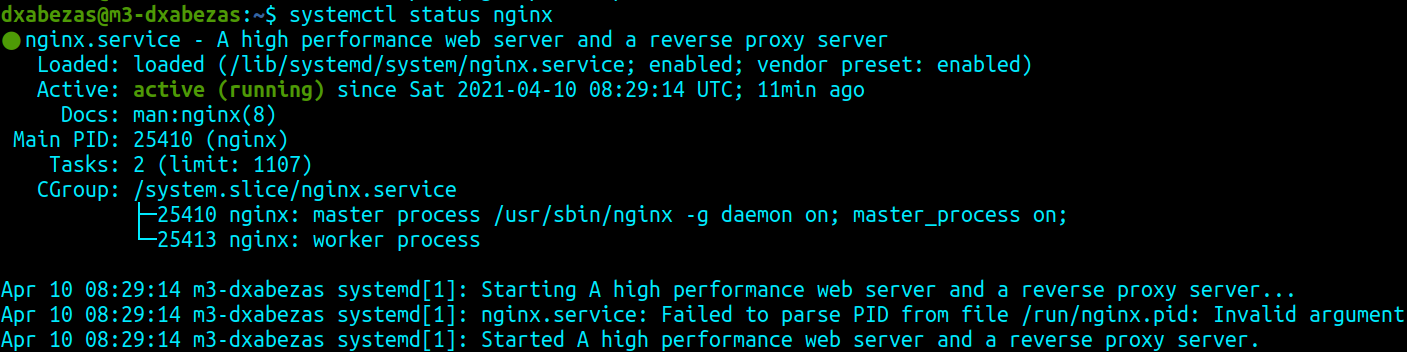
\includegraphics[width=148mm]{imgs/nginx-status}
	\caption{NGINX está activo.}
	\label{fig:nginx-status}
\end{figure}

Escribimos en \texttt{/etc/nginx/conf.d/default.conf} la configuración que se indica en el guión
para que NGINX funcione como balanceador de carga en lugar de como servidor web.

\begin{Verbatim}[tabsize=4]
upstream balanceo_dxabezas {
	server 192.168.56.101;
	server 192.168.56.102;
}

server{
	listen 80;
	server_name balanceador_dxabezas;
	access_log /var/log/nginx/balanceador_dxabezas.access.log;
	error_log /var/log/nginx/balanceador_dxabezas.error.log;
	root /var/www/;

	location \
	{
		proxy_pass http://balanceo_dxabezas;
		proxy_set_header Host $host;
		proxy_set_header X-Real-IP $remote_addr;
		proxy_set_header X-Forwarded-For $proxy_add_x_forwarded_for;
		proxy_http_version 1.1;
		proxy_set_header Connection "";
	}
}
\end{Verbatim}

Reestauramos el servicio con \verb^sudo service nginx restart^. Ahora si visitamos la IP de M3
en el navegador de la máquina anfitriona, observamos que NGINX sigue funcionando como servidor
web.

\begin{figure}[H]
	\centering
	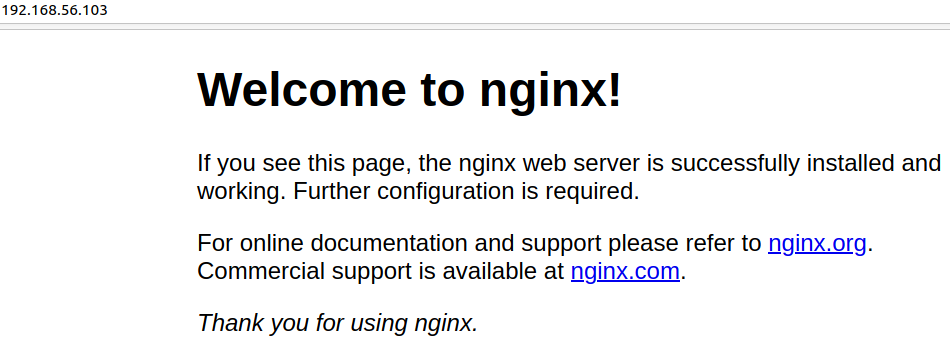
\includegraphics[width=100mm]{imgs/nginx-web}
	\caption{NGINX está funcionando como servidor web.}
	\label{fig:nginx-web}
\end{figure}

Como se nos indica en el guión, comentamos la línea \verb^/etc/nginx/sites-enabled/*;^
del fichero \texttt{/etc/nginx/nginx.conf}.

\end{document}
